\documentclass[732,14pt]{studrep}

\RequirePackage{tabularx}
% \RequirePackage{graphicx}
% Тестирование изменений
% \usepackage{showframe}

% test 

% pygmetize 
\RequirePackage{minted}
\RequirePackage{indentfirst}
\RequirePackage{graphicx}
\usemintedstyle{tango} % bw
\RequirePackage{doi}

% \setmainfont{Times New Roman}
\graphicspath{{pics/}}


\setminted{autogobble,mathescape,linenos=true,fontsize=\small,breaklines}
\begin{document}
\thispagestyle{empty}
\clearpage
 
\tableofcontents

\chapter*{ВВЕДЕНИЕ}
\label{chap:intro}
% TODO: Add contents line

\chapter{Методики прогнозирования состояния береговой зоны}\label{chap:techniques}




Таким образом, для обеспечения возможности проведения научных исследований в области инженерной геологии береговых зон водохранилищ необходимо создать ресурсы хранения информации и вычислительные ресурсы, обеспечивающие продуктивную среду прогнозирования с использованием различных математических моделей. .... модели предназначены для решения задач и ранжируются по видан задач, масштабу исследуемого объекта, размеру интервала времени, степени точности.

\chapter{Проектирование ГИС для прогнозирования береговой зоны}\label{chap:proj}

Анализ предметной области, представленный в Главе~\ref{chap:proj}, показал, что для получения качественно новых результатов научных исследований в инженерной геологии береговых зон внутренних водоемов, необходимо создать ресурсы хранения, преобразования, обеспечения эффективного доступа к этой информации, а также ее визуализации. Данные требования реализуются в виде информационно-вычислительную инфраструктуры, включающей набор сервисов (серверов), взаимодействующих согласно согласованному плану решения задачи. 

\section{Проектирование информационно-вычислительной среды}
\subsection{Функциональные требования}


... Необходимо обеспечить доступ к данным из разных ГИС (QGIS, ArcGIS и др.). Современные ГИС позволяют обеспечивать доступ пространственно-распределенным данным, представленным в специальных форматах, данным баз реляционных данных, а также виртуальных географических сервисов.

\subsection{Архитектура системы}
Перечисленные в предыдущем разделе функции формируют собой элементы архитектуры распределенной системы обработки ГИС-данных (рисунок~\ref{fig:arch}).

\begin{figure}
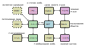
\includegraphics[width=0.7\linewidth]{pics\arch-p.svg}
  \caption{Архитектура распределенной системы} \label{fig:arch}
\end{figure}

Система состоит из двух основных частей, обычно обозначаемых как “клиент” и “сервер”. В нашем случае они взаимодействуют друг с другом по протоколу HTTP и реализуют взаимодействие через интерфейс “архитектуры REST” (Representation State Protocol). QGIS и ArcGIS - это клиентская часть, она включает также процедуры DSAS, ShRec (распознавание контура), ExpEv (экспертная оценка). QGIS также выступает клиентом для сервера изображений (формат JPG, TIFF, JP2 и др.), получаемых, в том числе, с сервера Google Maps. 

Серверная часть -- набор модулей, запускаемых удаленно из модуля \verb|shore_qgis_module|, т.е. процедурами распознавания управляет полностью   клиентская часть. Управление осуществляется через интерфейс REST, где в качестве объектов выступают сервисы хранения исходных изображений (OCV2 + HDF5), распознавания объектов на изображении (SegAny), анализ масок и изображений с целью получения дополнительных характеристик (FeatEx), сервис выгрузки данных с представлением в JSON (внутри REST). Приведем пример реализации интерфейсов REST для загрузки изображений и управления процессом распознавания.

\subsection{Интерфейс REST загрузки и обработки изображений}
Задача данного программного объекта - принимать бинарный файл изображения, преобразовать его в матрицы слоев, записать в базу данных на сервере, выдать глобальный идентификатор, при помощи которого далее идентифицируется сохраненные данные изображения.
\begin{minted}{python}
img = Service(name='imgstore',
              path='/sa-1.0/image/{img_name}',
              description="Image collection")

@img.put()
def put_image(request):
    """Принимает бинарные данные картинки,
    возвращает JSON с UUID сохраненного изображения
    """
    name = request.matchdict['img_name']

    imgg, ds = add_image(name, request.body)

    uui = uuidgen()
    uuis = str(uui)
    pth = ds.name
    STORAGE, INGRP, UUIDGRP = storage_begin()
    if name in UUIDGRP:
        ouuis = gs(UUIDGRP[name])
        del UUIDGRP[name]
        del UUIDGRP[ouuis]
    # Отображение UUID <-> имя изображения
    UUIDGRP.create_dataset(name, data=uuis)
    UUIDGRP.create_dataset(uuis, data=name)
    STORAGE, INGRP, UUIDGRP = storage_end()
    return {
        "error": None,
        "ok": True,
        "uuid": uuis,
        "content": pth,
        "name": name,
        "namepath": imgg.name
    }

def add_image(name, content, replace=True):
    ”””Добавление изображения в БД”””
    nparr = np.frombuffer(content, np.uint8)
    image = cv2.imdecode(nparr, cv2.IMREAD_COLOR)
    image = cv2.cvtColor(image, cv2.COLOR_BGR2RGB)
    # Открытие БД
    STORAGE, INGRP, UUIDGRP = storage_begin()
    if name in INGRP:
        del INGRP[name]
    imgg = INGRP.create_group(name)
    ds = imgg.create_dataset('content',
              data=image, compression="lzf")
    log.info("Image '{}' loaded".format(name))
    # Закрытие БД
    STORAGE, INGRP, UUIDGRP = storage_end()
    return (imgg, ds)
\end{minted}
Загрузка изображения делается при помощи запроса PUT с адресом \texttt{https://<адрес сервера>:6543/sa-1.0/image/<имя картинки>}. В тело запроса PUT помещается содержимое изображения. В качестве результата возвращается JSON-ответ, содержащий в поле “uuid” идентификатор сохраненного изображения. Список сохраненных изображений получается запуском запроса GET к этому же адресу без указания имени изображения. Возвращается JSON со списком отображений UUID-<имя файла изображения>. Полученный идентификатор используется для обозначения изображения, подвергающегося процедуре распознавания:

\begin{minted}{python}
sactrl = Service(name='segment-any-control',
                 path='/sa-1.0/sa/{img_uuid}/{cmd}',
                 description="Functions of SA on a image\
                              identified by uuid")
@sactrl.post()
def start_recognition(request):
    # Импорт процедур анализа, выполняющихся в
    #  других процессах
    from ..tasks import (sa_start, 
          ANSWERS, rc_set, rc_get, rc_delete,
          rc_update)

    uuids = request.matchdict['img_uuid']
    cmd = request.matchdict['cmd']
    # cmd = 'start'

    STORAGE, INGRP, UUIDGRP = storage_begin()
    # идентификатор изображения существует?
    isimg = uuids in UUIDGRP
    STORAGE, INGRP, UUIDGRP = storage_end()

    rd = {"error": False, "ok": True, "cmd": cmd}

    if cmd == "flush":
        ANSWERS.flushdb()
        return rd

    if not isimg:
        return {
            "error": "not found",
            "ok": False,
            "uuid": uuids,
            "cmd": cmd,
            "processuuid": None
        }
    # Команда запуска процесса распознавания
    if cmd == "start":
        prevrc = rc_get(uuids)
        if prevrc is not None:
            return {
                "error": "already running",
                "ok": False,
                "uuid": uuids,
                "cmd": cmd,
                "processuuid": prevrc.get("processuuid",
                                           None),
                "ready": prevrc.get("ready", False)
            }
        del prevrc
        rc = {"uuid": uuids, "ready": False}
        rc_set(uuids, rc)
        arc = sa_start.delay(uuids)
        puuid = str(arc.id)

        def _u(r):
            r["processuuid"] = puuid

        rc = rc_update(uuids, _u)
        print(rc_get(uuids))
        puuid = rd["processuuid"] = puuid
    # Команда проверки завершения процесса
    elif cmd == "status":
        rd["ready"] = False

        def _a(v, rr):
            rd["ready"] = v
            rd["result"] = rr.get("result", None)

        rc = rc_get(uuids, "ready", _a)
        if rc is None:
            return {
                "error": "no process",
                "ok": False,
                "uuid": uuids,
                "cmd": cmd,
                "ready": None
            }

        rd["processuuid"] = rc["processuuid"]
    # Команда завершения процесса и удаления его данных
    elif cmd == "finalize":
        rcg = rc_get(uuids)
        if rcg is None:
            return {
                "error": "not running",
                "ok": False,
                "uuid": uuids,
                "cmd": cmd,
                "ready": None
            }
        rc_delete(uuids)
        rd.update({"ready": rcg["ready"], 
                   "processuuid": rcg["processuuid"]})
    # Команда отмены процесса
    elif cmd == "discard":
        rcg = rc_get(uuids)
        if rcg is not None:
            return {
                "error": "still running",
                "description":
                "cannot stop SA, wait its finishing. \
                     Use status command.",
                "ok": False,
                "uuid": uuids,
                "cmd": cmd,
                "ready": None
            }
        STORAGE, INGRP, UUIDGRP = storage_begin()
        name = gs(UUIDGRP[uuids])
        imgg = INGRP[name]
        if "masks" in imgg:
            del imgg["masks"]
            rc = "removed"
        else:
            rc = "no mask"
        STORAGE, INGRP, UUIDGRP = storage_end()
        rd.update({
            "ready": None,
            "processuuid": None,
            "description": rc
        })

    return rd
\end{minted}

Запуск процесса распознавания осуществляется при помощи запроса POST следующего формата - \texttt{http://<адрес сервера>:6543/sa-1.0/sa/<идентификатор изображения>/<команда>}. Командой выступает ключевое слово - одно из четырех:
\begin{description}
  \item[start] -- запуск нового процесса, 
  \item[status] -- запрос состояния распознавания,
  \item[finalize] -- завершение исполнившегося процесса,
  \item[flush] -- отмена процесса.
\end{description}
Требующие большие вычислительные ресурсы процессы выполняются в отдельных процессах сервера или на специализированных серверах, снабженных аппаратной поддержкой вычислений (CUDA и ему подобным). Реализация запуска таких задач реализована при помощи библиотеки celery языка программирования Python.

\chapter{Реализация подсистем распределенной вычислительной среды}\label{chap:impl}


\section{Тестирование}

\chapter*{ЗАКЛЮЧЕНИЕ}

Выпускная квалификационная работа посвящена проекту развития научного направления Лаборатории инженерной геологии и геоэкологии в аспекте повышения уровня информатизации и обработки данных полевых исследований. В работе решены следующие задачи:
\begin{enumerate}
  \item Проведена формализация предметной области инженерной геологии, относящейся к исследованиям экзогенных геологических процессов на берегах крупного внутреннего водоёма, представлена концептуальная модель в виде онтологии,
  \item Разработана информационно-вычислительной инфраструктура поддержки прогнозирования состояния береговой зоны на основе геоинформационной системы и распределенной вычислительной среды,
  \item Предложен вариант архитектуры вычислительной среды,  реализованы некоторые её подсистемы с использованием современных средств автоматизации распознавания объектов на изображениях,
  \item Для реализованных подсистем предложены модели данных, предназначенных для хранения информации в процессе её обработки,
  \item Продемонстрирована работоспособность предложенной среды на простом примере прогнозирования.
\end{enumerate}

Рассмотренные в диссертации вопросы преследуют целью формирование вычислительных ресурсов поддержки принятия решений по результатам мониторинга, оценки и прогноза опасных геологических процессов. Дальнейшее направление научных исследований и опытно-конструкторских работ имеет смысл продложать по нескольким основным направлениям:
\begin{itemize}
  \item Завершение реализации информационно-вычислительный среды,
  \item Наполнение информационных ресурсов архивными данными и данными современного мониторинга объектов исследования,
  \item Совершенствование методов прогнозирования состояния береговой зоны за счет реализации современного уровня информационного обеспечения,
  \item Разработка экспертной системы оценки результатов моделирования с целью формирования рекомендаций по использованию конкретных участков исследуемой береговой зоны.
\end{itemize}



      

\begin{thebibliography}{99}
  

  \bibitem{gruber} Gruber, T. Toward Principles for the Design of Ontologies Used for Knowledge Sharing. International Journal of Human-Computer Studies. 43 (5–6): 907–928. doi:10.1006/ijhc.1995.1081. S2CID 1652449.

Thomas R. Gruber,
Toward principles for the design of ontologies used for knowledge sharing?,
International Journal of Human-Computer Studies,
Vol. 43, No. 5–6,
1995,
Pp. 907-928,
ISSN 1071-5819,
\doi{10.1006/ijhc.1995.1081}, \url{https://www.sciencedirect.com/science/article/pii/S1071581985710816} (дата доступа: 11.05.2024)
\end{thebibliography}




\end{document}
